\documentclass{article}

\usepackage[utf8]{inputenc}
\usepackage{amssymb}
\usepackage{amsmath} 
\usepackage{enumitem}
\usepackage{pgf,tikz}
\usepackage{tkz-euclide}
\usepackage{mathrsfs}
\usepackage{xcolor}
\usetikzlibrary{arrows}
\usepackage{fancyhdr}
\usepackage{hyperref}
\usepackage{wrapfig}
\usepackage{polski}
\usepackage{pgfplots}
\usepgfplotslibrary{external}
\usepackage{gensymb}
\usepackage[many]{tcolorbox}
\usepackage{mathtools}
\PassOptionsToPackage{hyphens}{url}
\usepackage{xurl}
\usetikzlibrary{patterns}

\pagestyle{empty}

% definicja koloru
\definecolor{kolor}{RGB}{8, 97, 138}

\DeclareUnicodeCharacter{2212}{-}

% definicja kąta
\def\an{\hbox{\lower-.2ex\hbox{$<\kern-.53em)$}$\,$}}

\usepackage[b5paper, left=0.8in, right=0.8 in, top=0.8 in, bottom=0.8 in]{geometry}

\usetikzlibrary{arrows, calc,intersections, decorations.pathmorphing}
\tikzset{
arrowMe/.style={postaction=decorate,
    decoration={markings, mark=at position .5 with {\arrow[thick]{#1}}
    } }}


\newcommand{\heading}[1]{
  \noindent
  \textbf{\textcolor{kolor}{#1}}
  \vspace{5px}
}

\newcommand{\remark}{
  \noindent\textit{Uwaga}\\
}

\newcommand{\theory}[1]{
  \addcontentsline{toc}{subsection}{#1}
	\begin{center}
    \fontsize{26}{20}\selectfont
	\textbf{\textcolor{kolor}{#1}}
	\end{center}
	\vspace{20px}
}

\tcbset{mystyle/.style={
  breakable,
  enhanced,
  outer arc=0pt,
  arc=0pt,
  colframe=kolor,
    coltitle=kolor,
  colback=white,
  attach boxed title to top left={yshift=-2mm},
  boxed title style={
    coltitle=kolor,
    colback=white,
    outer arc=0pt,
    arc=0pt,
    top=3pt,
    bottom=3pt,
    },
  fonttitle=\sffamily
  }
}

\newtcolorbox[auto counter]{problem_box}[1][1]{
  mystyle,
  title=Zadanie~{#1},
}


\newlist{hints_list}{enumerate}{3}

\setlist[hints_list]{label=\textbf{\textcolor{kolor}{\arabic*}}.}

\newcommand{\hints}[1]{
  \addcontentsline{toc}{subsection}{#1}
  \vspace{10px}
  \begin{center}
    \fontsize{20}{20}\selectfont
  \textbf{\textcolor{kolor}{#1}}
  \end{center}
}

\newcommand{\sources}[1]{
  \vspace{20px}
  \addcontentsline{toc}{subsection}{#1}
  \vspace{10px}
  \begin{center}
    \fontsize{20}{20}\selectfont
  \textbf{\textcolor{kolor}{#1}}
  \end{center}
  \vspace{10px}
}

\newcommand{\source}[1]{
\noindent
  \textbf{\textcolor{kolor}{#1}} \; 
  \noindent
}

\newcommand{\solutions}[1]{
  \addcontentsline{toc}{subsection}{#1}
	\begin{center}
    \fontsize{26}{20}\selectfont
	\textbf{\textcolor{kolor}{#1}}
	\end{center}
	\vspace{20px}
}


\newenvironment{problem}[1]
{
    \begin{samepage}
    \begin{problem_box}[{#1}]
}
{ 
    \end{problem_box}
    \end{samepage}
}

\newcommand{\answer}[1]{
  \noindent\textit{Odpowiedź.} #1
  \vspace{5px}
}

\newcommand{\headingpage}[1]{
\newpage
  \vspace*{\fill}
  \begin{center}
    \fontsize{30}{30}\selectfont
    \textcolor{kolor}{#1}
  \end{center}
\vspace*{\fill}
\newpage
}



\newcommand{\rotatehint}[1]{
\vspace{1 px}\noindent\scriptsize{\rotatebox{180}{Podpowiedź: #1}}\normalsize
\vspace{5px}}

\newcommand{\qed}{\hfill $\blacksquare$}


\begin{document}


\noindent
Pokolorujmy ten prostokąt w szachownicę. Załóżmy, że lewe dolne pole będzie koloru czarnego. Skoro prostokąt $\mathcal{P}$ ma bok nieparzystej długości, to wszystkie jego narożne pola będą koloru czarnego. Również zawiera on o jedno pole czarne więcej niż zawiera pól białych. 

\vspace{10px}
\noindent
Każdy z prostokątów, na które jest on podzielony można zaklasyfikować do jednego z trzech typów:
\begin{itemize}
	\item Prostokąt, który ma dwa pola narożne białe i dwa pola narożne czarne. Zawiera on tyle samo pól białych, co czarnych;
	\item Prostokąt o czterech polach narożnych białch. Zawiera on o jedno pole białe więcej;
	\item Prostokąt o czterech polach narożnych czarnych. Zawiera on o jedno pole czarne więcej.
\end{itemize}

\begin{center}
	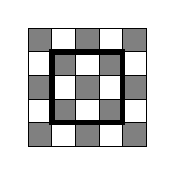
\begin{tikzpicture}[scale=0.3]

		\fill[color=gray] (0,0) rectangle (1,1);
		\fill[color=gray] (1,1) rectangle (2,2);
		\fill[color=gray] (2,2) rectangle (3,3);
		\fill[color=gray] (3,3) rectangle (4,4);
		\fill[color=gray] (4,4) rectangle (5,5);
		\fill[color=gray] (0,4) rectangle (1,5);
		\fill[color=gray] (0,2) rectangle (1,3);
		\fill[color=gray] (1,3) rectangle (2,4);
		\fill[color=gray] (2,4) rectangle (3,5);
		\fill[color=gray] (2,0) rectangle (3,1);
		\fill[color=gray] (3,1) rectangle (4,2);
		\fill[color=gray] (4,2) rectangle (5,3);
		\fill[color=gray] (4,0) rectangle (5,1);

		\draw (0,0) -- (5,0) -- (5,5) -- (0,5) -- cycle;
		\draw (0,1) -- (5,1);
		\draw (0,2) -- (5,2);
		\draw (0,3) -- (5,3);
		\draw (0,4) -- (5,4);


		\draw (1,0) -- (1,5);
		\draw (2,0) -- (2,5);
		\draw (3,0) -- (3,5);
		\draw (4,0) -- (4,5);

		\draw[line width=2pt] (1,1) rectangle (4,4);
		
	\end{tikzpicture}
\end{center}

\noindent
Skoro $\mathcal{P}$  zawiera o jedno pole czarne więcej, to pewien z rozpatrywanych prostokątów, nazwijmy go $P$ musi mieć czarne pola narożne. Zarówno $\mathcal{P}$, jak  $P$ mają czarne pola narożne, z czego łatwo wynika, że odległości między odpowiadającymi im bokami są tej samej parzystości.

\end{document}